%\documentclass[12pt, oneside]{article}
\documentclass[review]{elsarticle}
\usepackage{hyperref}
%\usepackage{lineno,hyperref}
%\modulolinenumbers[5]
%\includegraphics
\usepackage[margin=1in]{geometry}
%\geometry{letterpaper}
%\usepackage[parfill]{parskip}
\usepackage{graphicx}
\usepackage{amsmath}
%\usepackage{authblk}
%\usepackage{amssymb}
%\usepackage{cite}
%\usepackage{float}
%\usepackage{fixltx2e}
\usepackage{placeins}
%\usepackage{verbatim}
\usepackage{comment}
\usepackage{gensymb}


\journal{Journal of Nuclear Materials}
\bibliographystyle{elsarticle-num}

\begin{document}
\begin{frontmatter}
\title{Threshold displacement energy of $\alpha$ and $\gamma$ uranium}

\author[inl]{Benjamin Beeler\corref{qwe}}
\cortext[qwe]{Corresponding author}
\ead{benjamin.beeler@inl.gov}
\author[inl]{Yongfeng Zhang}
\address[inl]{Idaho National Laboratory, Idaho Falls, ID 83415}

\begin{abstract}
A monolithic fuel design based on a U-Mo alloy has been selected as the fuel type for conversion of the United States High-Performance Research Reactors (HPRRs) from highly enriched uranium (HEU) to low-enriched uranium (LEU). In this fuel design, there exists a variable degree of phase decomposition from the body-centered cubic $\gamma$ phase of uranium to the orthorhombic $\alpha$ phase of uranium depending on molybdenum content and fabrication conditions. These two phases are believed to exhibit distinct swelling and radiation damage behavior. Understanding the differences in behavior between the $\alpha$ and $\gamma$ phases can provide valuable information to guide the manufacturing process of U-Mo alloys and can inform multiphysics, continuum-level fuel performance codes. The threshold displacement energy (TDE) is the minimum amount of kinetic energy required to displace an atom from its lattice site. It is critically important to determine an accurate value of the TDE in order to calculate the total number of displacements due to a given irradiation condition, and thus to understand the materials response to irradiation. In this study, molecular dynamics simulations have been performed to calculate the threshold displacement energy for both the $\alpha$ and $\gamma$ phases of uranium. 
\end{abstract}
\end{frontmatter}

%\linenumbers

\section{Introduction}

In the interest of nuclear non-proliferation, there has been renewed interest in recent decades to replace current highly enriched uranium (HEU) fuel in high power research reactors with low enriched uranium (LEU) fuel \cite{snelgrove1997}. In the United States, this program is the United States High-Performance Research Reactor (USHPRR) program. Research reactors require fuel that operates at high power and reaches high fission density, but at relatively low temperatures. Typical research reactor fuel consists of aluminum (Al) cladding surrounding a fuel meat composed of fuel particles dispersed in an Al matrix \cite{meyer2014}. In order to achieve a reduced enrichment in these fuel types, there is a requirement for increased uranium density. One way this is achieved is by utilizing $\gamma$ stabilized uranium alloys with 10 wt.\% or less alloy content. The fuel design being pursued under the USHPRR program is a uranium-molybdenum (U-Mo) monolithic foil, with a zirconium (Zr) diffusion barrier in Al clad, as shown in Figure \ref{fig:ben1}. 

\begin{figure}[!h]
 \centering
 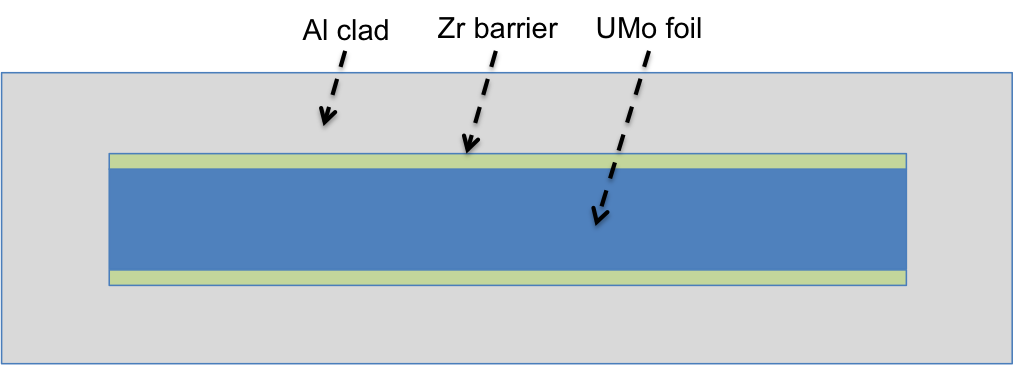
\includegraphics[width=0.8\textwidth]{ben1.png} % requires the graphicx package
 \caption{Schematic of U-Mo monolithic fuel cross section. Not to scale.}
 \label{fig:ben1}
\end{figure}

\FloatBarrier

One issue with metallic fuels, including UMo fuels, is the large amount of swelling that takes place \cite{hofman1997}. Such swelling can be accounted for in the fuel design, however the swelling needs to be stable and predictable up to high fission densities. Research reactor fuel types are unique in that there cannot exist fission gas release from the fuel, and as such there is a relatively high content of fission gas and of fission gas bubbles within the fuel matrix. This importance of swelling in addition to the unique fuel environment has led to a variety of studies attempting to characterize the swelling behavior in U-Mo fuels \cite{rest2009, kim_anl08, meyer2002, kim2013} which has led to the development of a swelling correlation from Argonne National Labortory (ANL correlation) \cite{kim2011} as a function of fission density. This swelling correlation was intended to be applicable for low temperature (less than 250$^{\circ}$C) U-Mo alloys in the 7-10 wt.\% composition range. 

A 2015 post-irradiation examination (PIE) report \cite{afip6report} showed early onset break-away swelling in U-10Mo fuels at fission densities much lower than previously observed. This fuel swelling behavior deviated from the ANL correlation and such behavior could lead to early fuel failure. Understanding the cause of this anomalous swelling behavior is a critical step in qualifying U-Mo fuel for use in research reactors. This PIE report showed a large amount of compositional banding, or regions of low Mo content adjacent to regions of higher Mo content. An increased amount of swelling was also observed in lower Mo content alloys (U-7Mo) \cite{vandenberghe2014} at lower fission densities. Lower Mo content leads to phase transformation from the $\gamma$ U-Mo body-centered cubic phase to the $\alpha$ U phase \cite{janfong2014}. This is most evident in the region involving the U-Mo fuel foil and the Zr diffusion barrier \cite{park2015}. Near the Zr diffusion barrier, there exists a limited region of interaction where there exists a variety of phases including $\gamma$ U-Mo, UZr$_{2}$, Mo$_{2}$Zr and $\alpha$ U. This interdiffusion region exhibits the highest density of fission gas bubbles at high fission densities and is the region where fuel separation initiates \cite{rertr12}. Finally, in alloys with either lower Mo content or increased banding, it has been observed an earlier onset of recrystallization \cite{kim2013A}. Recrystallization is the suggested culprit behind break-away swelling, as the recrystallized grains are destroying the fission gas superlattice \cite{vandenberghe2008}. This information suggests that there is a fundamental difference between the radiation damage behavior and swelling behavior of the $\alpha$ phase of U and the $\gamma$ phase of U-Mo. The first step to unraveling this puzzle is to investigate the radiation damage-related properties of both $\alpha$ U and $\gamma$ U.

One of the most fundamental quantities of radiation damage is the threshold displacement energy (TDE). The TDE is defined as the minimum amount of kinetic energy required to displace an atom from its lattice site. This quantity plays a key role in radiation damage theory, where it is implemented within the Kinchin-Pease \cite{kinchinpease} or the Norgett-Robinson-Torrens (NRT) \cite{norgett1975} equations, which state that the amount of damage is proportional to the ratio of the amount of deposited energy to an effective TDE. Therefore, it is critically important to determine an accurate value of the TDE in order to calculate the total number of displacements due to a given irradiation condition, and thus understand the materials response to irradiation.

In this paper, molecular dynamics (MD) simulations have been performed to calculate the TDE in $\alpha$ and $\gamma$ U at 600 K, 800 K and 1000 K utilizing three unique interatomic potentials. The probability of Frenkel pair production is determined as a function of PKA direction and temperature. Probability curves are averaged to determine an effective value of the TDE, above which a Frenkel pair is more than 50 $\%$ likely to form. 

\section{Computational Details}
In order to determine the TDE at temperatures of interest for nuclear reactors, molecular dynamics (MD) \cite{abraham1986, allen1987} simulations need to be performed. MD requires an interatomic potential to describe the energy landscape of the system being studied. Very few interatomic potentials have been constructed for uranium-based alloys. This is due to the inherent difficulty in describing the behavior of f-electrons and the mechanical instability of the $\gamma$ phase of uranium at low temperatures. Several interatomic potentials have been developed for pure uranium \cite{beeler_meam, beelerASTM, fernandez2014, li2011, smirnova2012, li2012}, with only a few being adapted into alloy potentials for U-Zr \cite{moore2015}, U-Al \cite{pascuet2012} and U-Mo \cite{smirnovaUMo}. The modified Embedded-Atom Method (MEAM) variants of U and U-Zr \cite{beeler_meam, moore2015} are the two potentials that can most accurately describe the $\gamma$ phase of uranium, and the pure U MEAM potential \cite{beeler_meam} has been utilized for a prior radiation damage study \cite{miao2015}. However, the pure U MEAM potential is incapable of accurately describing the $\alpha$ phase. The U-Zr variant of the MEAM potential is an updated version of the prior pure MEAM potential that had been modified to accurately describe a variety of alloy properties of $\gamma$ U-Zr. The U-Mo ADP \cite{smirnovaADP} potential can accurately describe the $\gamma$ U-Mo phase with the added benefit of being able to describe the $\alpha$ phase of U. Thus, to develop a full picture of the radiation damage behavior in $\alpha$ and $\gamma$ U with applicability to $\gamma$ U-Mo, all three potentials should be utilized and compared.

Molecular dynamics simulations are performed utilizing the LAMMPS \cite{plimpton1995} software package and the MEAM U \cite{beeler_meam}, MEAM UZr \cite{moore2015} and ADP UMo \cite{smirnovaADP} potentials splined to a Ziegler, Biersack and Littmark (ZBL) \cite{zbl} potential at small distances. To generate curves of the probability of Frenkel pair production as a function of PKA energy in $\alpha$U, a supercell containing 18,000 atoms is equilibrated for 200 ps at a given temperature in an NPT ensemble. The thermostat damping parameter is set to 1.7 ps to match the macroscopic thermal conductivity \cite{lane2012}. An atom is then given extra kinetic energy, with the velocity directed in varying prescribed directions. The time step is set to 0.2 fs and the simulation is run for 70,000 steps (14 ps). This time is long enough such that the thermal spike emanating from the cascade has dispersed, while allowing immediate recombination of defects. This time is also short enough such that substantial thermal diffusion has not occurred. The system is then quenched to 10 K for ease of defect analysis. The number of stable Frenkel pairs is determined via a Wigner-Seitz cell based algorithm \cite{hayward2010}. This simulation procedure is identical for $\gamma$U, excepting a supercell size of 16,000 atoms. 

PKA energies are varied over a range of approximately 150 eV, in steps of 10 eV, to properly sample the relevant energy range. In the $\gamma$ phase, the analysis includes 55 unique PKA directions that sample the body-centered cubic crystal cell \cite{beeler2015}. In the $\alpha$ phase, the analysis includes 64 unique PKA directions. The set of directions are determined by varying the angles $\theta$ and $\phi$ as shown in Fig \ref{fig:directions}. For the $\gamma$ phase, $\theta$ is varied from 0\degree to 90\degree and $\phi$ is varied from 0\degree to 45\degree. For the $\alpha$ phase, both $\theta$ and $\phi$ are varied from 0\degree to 90\degree. For each PKA direction, 100 independent simulations are performed, each simulation with an independent distribution of initial velocities. 

\begin{figure}[h]
 \centering
 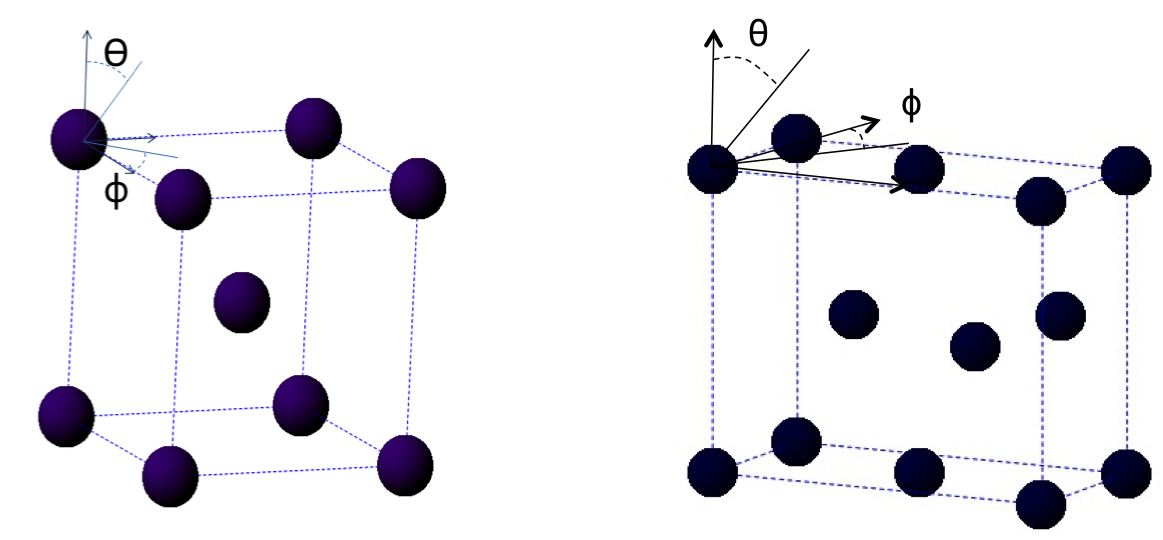
\includegraphics[width=0.8\textwidth]{directions.png} % requires the graphicx package
 \caption{The set of PKA directions are determined by varying the angles $\theta$ and $\phi$. For the $\gamma$ phase (left), $\theta$ is varied from 0\degree to 90\degree and $\phi$ is varied from 0\degree to 45\degree. For the $\alpha$ phase (right), both $\theta$ and $\phi$ are varied from 0\degree to 90\degree.}
 \label{fig:directions}
\end{figure}

\FloatBarrier

As reviewed by Nordlund \cite{nordlund2006}, several different definitions of TDE can be introduced. In the previous literature, the primary type of TDE reported is the E$^{\textrm{l}}_{\textrm{d}}$, or the lower bound of the displacement energy, where there exists a non-zero probability of creating a defect \cite{malerba2002}. Typically, the direct experimental measurements of the TDE measure the lowest energy where a defect signal can be detected, for example by changes in resistivity. This is analagous to the E$^{\textrm{l}}_{\textrm{d}}$. For comparison to experiment, adjustments for beam spreading should be included \cite{nordlund2006}. For implementation into the Kinchin-Pease or NRT equations, an average value for the TDE needs to be utilized that is distinct from E$^{\textrm{l}}_{\textrm{d}}$ \cite{nordlund2006,norgett1975}. This average value is obtained from generating probability curves (probability of generating a Frenkel pair as a function of PKA energy) for respective PKA directions. These probability curves can then be averaged over all directions to create an angle-integrated displacement probability curve \cite{nordlund2006}. The energy at which this averaged probability curve crosses the probability 0.5 is determined to be the median TDE (E$^{\textrm{pp}}_{\textrm{d,med}}$), where pp stands for production probability. This value takes into account not only displacement of atoms, but allows for subsequent recombination in the time-frame of the 14 ps simulation following the PKA event. This is the appropriate description of TDE for use in the NRT equation. Only the E$^{\textrm{pp}}_{\textrm{d,med}}$ is calculated in this work.

\section{Results}
\subsection{$\gamma$U Median Threshold Displacement Energy}
In this section, E$^{\textrm{pp}}_{\textrm{d,med}}$ in $\gamma$U is determined at 800 K and 1000 K. For each interatomic potential used (U MEAM \cite{beeler_meam}, UZr MEAM \cite{moore2015} and UMo ADP \cite{smirnovaADP}), the probability of Frenkel pair production as a function of PKA energy is generated for each unique PKA direction. This leads to 55 unique probability curves for each interatomic potential, given that there are 55 unique PKA directions investigated in $\gamma$U. To illustrate the nature of these curves, Fig \ref{fig:ed_dir} displays the probability curves for three different PKA directions utilizing the U MEAM interatomic potential in $\gamma$U at 800 K. The PKA directions are labeled as \textit{dir2}, \textit{dir24} and \textit{dir28}. The curves shown are fourth order polynomial fits to the data points collected (data points not shown for clarity). The first significant observation is that there is a wide discrepancy between each of the individual directions. The calculated E$^{\textrm{pp}}_{\textrm{d,med}}$ for each individual direction are 36 eV, 58 eV and 101 eV for \textit{dir2}, \textit{dir24} and \textit{dir28}, respectively. This shows a variance in the threshold energy of approximately 70 eV depending on the direction of the PKA. Such dramatic variance underlines the importance of gathering a large set of PKA directions to accurately sample the entire phase space of the crystal structure of interest such that true average behavior can be approximated. The second significant observation is that there are non-negligible probabilities of defect production over a wide range of PKA energies, as has been seen before in other materials \cite{beeler2016, nordlund2006}. This is most evident for \textit{dir24}, where probabilities vary from 0 at 20 eV, to 0.72 at 140 eV, with the PKA energy of 101 eV yielding a probability of 0.5. Such a large range of non-zero probabilities highlights that the TDE at high temperatures is far from the step-function-like description at 0 K \cite{was2007}. Finally, the probabilities become non-zero at approximately 20 eV for all three PKA directions. This suggests the E$^{\textrm{l}}_{\textrm{d}}$ near 20 eV for this system using this potential, although this value was not strictly determined in this work. 
 
\begin{figure}[h]
 \centering
 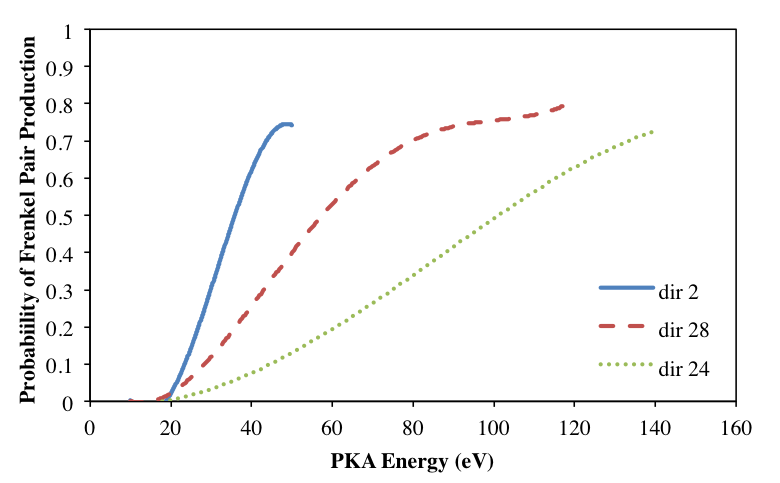
\includegraphics[width=0.8\textwidth]{ed_dir.png} % requires the graphicx package
 \caption{The Frenkel pair production probability curves in $\gamma$U at 800 K for the U MEAM interatomic potential in three different PKA directions.}
 \label{fig:ed_dir}
\end{figure}

\FloatBarrier

The probability curves for all PKA directions are arithmetically averaged, creating a single angle-integrated probability curve for each of the three interatomic potentials. These three angle-integrated probability curves are displayed in Fig. \ref{fig:gam800} for results at 800 K. In Fig \ref{fig:gam800} a line is overlaid on the data at a probability of 0.5 over the entire energy spectrum. The major observation from Fig. \ref{fig:gam800} is the significant difference in the results from each of the potentials. There exists a shift right of the curves moving from the UMo ADP to the UZr MEAM to the U MEAM, yielding lowest probabilities for the U MEAM for the same given PKA energy and highest probabilities for the UMo ADP. The value of E$^{\textrm{pp}}_{\textrm{d,med}}$ at 800 K calculated by the U MEAM potential is 74.5 eV; for the UZr MEAM potential, 47 eV; for the UMo ADP potential, 35.6 eV. Given that the number of displacements in the NRT equation \cite{norgett1975} is proportional to E$_{d}^{-1}$, comparing the E$^{\textrm{pp}}_{\textrm{d,med}}$ results for the U MEAM potential and the UMo ADP potential yields a factor of 2 difference in the total number of displacements. This discrepancy is dramatic and points to the importance of selection of interatomic potential, and awareness of the unique behaviors of the potential that is chosen when performing radiation damage simulations. Unfortunately, there does not exist experimental data on the displacement energy to determine the E$^{\textrm{pp}}_{\textrm{d,med}}$, and as such the determination of which interatomic potential is displaying accurate behavior is unavailable. 

\begin{figure}[h]
 \centering
 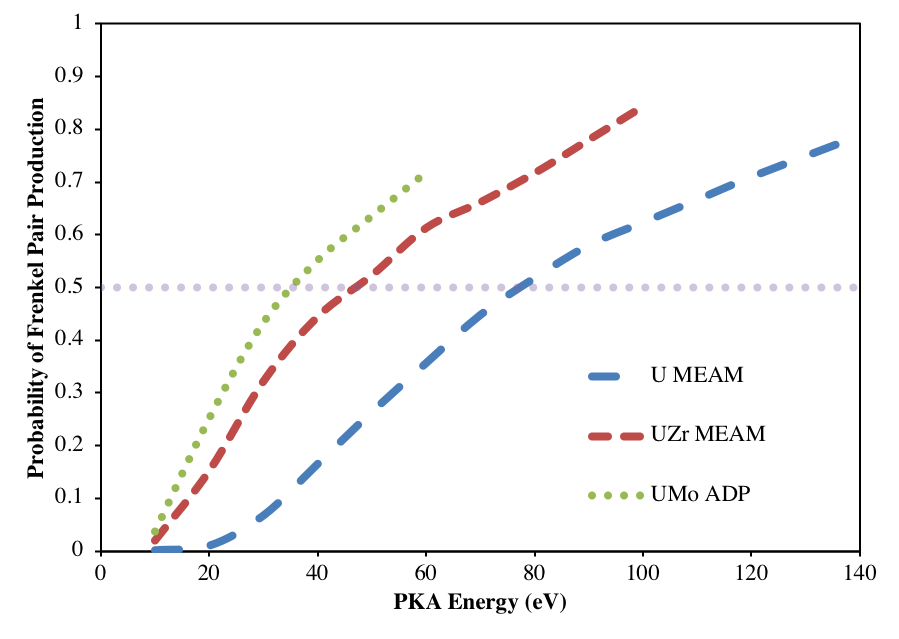
\includegraphics[width=0.8\textwidth]{gam800.png} % requires the graphicx package
 \caption{The angle-integrated Frenkel pair production probability curves in $\gamma$U at 800 K for three interatomic potentials.}
 \label{fig:gam800}
\end{figure}

\FloatBarrier

The next comparison to make is regarding the effect of temperature on the E$^{\textrm{pp}}_{\textrm{d,med}}$ for each given potential. The results at 800 K and 1000 K are summarized in Table \ref{tab:gam}. Included in Table \ref{tab:gam} in parentheses are a lower and upper bound. In order to determine the statistical significance of these results, the standard error of the mean was determined for each data point utilized to construct Fig. \ref{fig:gam800} and such curves for the system at 1000 K. The standard error of the mean for each data point was added to that respective data point in order to create a higher bound probability curve. Likewise a lower bound probability curve was created by subtracting the standard error of the mean for each respective data point. The upper bound and lower bound E$^{\textrm{pp}}_{\textrm{d,med}}$ is calculated from the point where the upper bound and lower bound probability curves, respectively, cross 0.5 probability. This can provide us with a most probable range (68.2\% confidence interval) for the values of E$^{\textrm{pp}}_{\textrm{d,med}}$. These ranges are provided in Table \ref{tab:gam} in parentheses. 

\begin{table}[h]
\caption{The median threshold displacement energy in $\gamma$U for three different potentials and two temperatures. Energies given in eV. A range incorporating plus/minus one standard error is included in parentheses for each system.} \label{tab:gam}
\begin{center}
\begin{tabular}{|c|c|c|}
	\hline
	& 800 K & 1000 K \\
	 \hline
	 U MEAM & 74.5 (72.9-80.8) & 68.8 (66.4-71.3) \\
	 UZr MEAM & 47.0 (44.5-49.5) & 41.3 (39.8-42.8) \\
	 UMo ADP & 35.6 (33.9-37.4) & 32.8 (31.8-33.7) \\
	 \hline
\end{tabular}
\end{center}
\label{default}
\end{table}

\FloatBarrier

For all three potentials, there is observed a decrease in the magnitude of the E$^{\textrm{pp}}_{\textrm{d,med}}$ as temperature increases from 800 K to 1000 K. Previous work performed by the authors have shown the opposite trend in body-centered cubic (bcc) Fe: an increase in the E$^{\textrm{pp}}_{\textrm{d,med}}$ with increasing temperature \cite{beeler2016}. In bcc Fe, this is explained via higher temperatures leading to greater recombination rates, and thus an increase in the difficulty of creating defects that last longer than a few picoseconds after the dissipation of the thermal spike. Another previous study in bcc Fe \cite{beeler2015, beeler2016} showed that trends of the formation energy of Frenkel pairs as a function of applied strain were linked to the threshold displacement energy as a function of applied strain. Thus, an investigation into defect formation energy trends versus temperature for metallic uranium was undertaken in an attempt to explain these results. Frenkel pair formation energies were determined by equation \ref{eqn:eint}.

\begin{equation}
\label{eqn:eint}
E_{f}^{int} = E_{int} + E_{vac} - 2*E_{pure}
\end{equation} 

where E$_{int}$ is the energy of a system with an interstitial, E${vac}$ is the energy of a system with a vacancy and E$_{pure}$ is the energy of a pure system consisting. E$_{pure}$, E$_{vac}$ and E$_{int}$ were determined by conducting 10 unique simulations for each system. In each simulation, the system is equilibrated for 1 ns at a prescribed temperature, wherein the energy is averaged over the final 500 ps of the simulation. The resultant energy from each of the 10 simulations was averaged to calculate E$_{pure}$, E$_{vac}$ and E$_{int}$. The results from 800 K to 1200 K in intervals of 100 K are displayed in Table \ref{tab:eform}. Due to statistical fluctuations at high temperatures, there exists an amount of error associated with conducting these simulations. This is the reasoning behind conducting multiple simulations and averaging over the produced set of data. The standard error is calculated as the standard deviation of a set divided by the square root of the sample size. The total error in the formation energy is a sum of the standard error for the 10 simulations for E$_{pure}$, the standard error for the 10 simulations for E$_{vac}$ and the standard error for the 10 simulations for E$_{int}$. The data in Table \ref{tab:eform} is illustrated in Fig \ref{fig:eform}, on which error bars are included. 

For all three potentials, the Frenkel pair formation energy increases from 800 K to 1000 K and generally as a function of temperature. This would suggest an increase in the threshold displacement energy from 800 K to 1000 K, however, the opposite trend is observed in Table \ref{tab:gam}. Thus, there is another factor dominating the temperature trends in the threshold displacement energy other than Frenkel pair formation energy. Since we know that increase in temperature yields increases in diffusion, it is worthwhile to investigate the diffusion coefficients and the migration barriers of defect diffusion in $\gamma$U for each of these three potentials over temperatures of interest. Some diffusion studies have been performed utilizing these potentials \cite{smirnovaADP}, but not for all three potentials, and the results were not fully quantified. 

\begin{table}[h]
\caption{The Frenkel pair formation energy in $\gamma$U for three different potentials from 800 K to 1200 K. Energies given in eV.} \label{tab:eform}
\begin{center}
\begin{tabular}{|c|c|c|c|c|c|}
	\hline
	& 800 K & 900 K & 1000 K & 1100 K & 1200 K\\
	 \hline
	 U MEAM & 2.35 & 2.44 & 2.88 & 3.14 & 3.05 \\
	 UZr MEAM & 2.81 & 3.44 & 3.67 & 3.66 & 4.05 \\
	 UMo ADP & 3.00 & 2.88 & 3.27 & 3.31 & 3.52 \\
	 \hline
\end{tabular}
\end{center}
\label{default}
\end{table}

\begin{figure}[h]
 \centering
 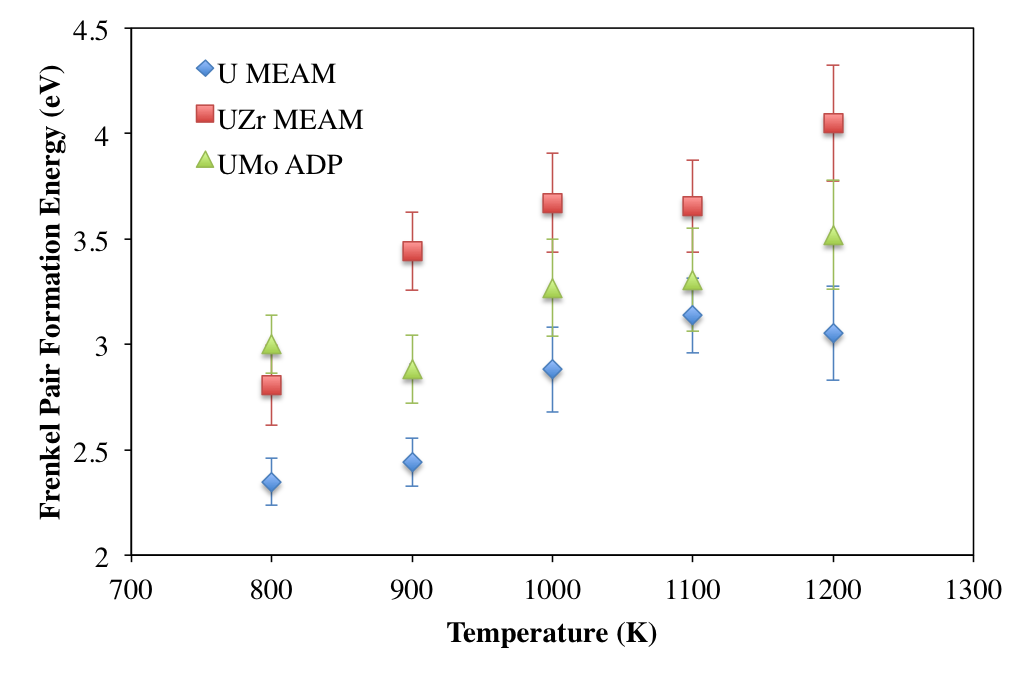
\includegraphics[width=0.8\textwidth]{frenkel_eform.png} % requires the graphicx package
 \caption{The Frenkel pair formation energy in $\gamma$U for three different potentials from 800 K to 1200 K. Error bars denote plus/minus one standard error.}
 \label{fig:eform}
\end{figure}

\FloatBarrier

Utilizing the same simulations that were performed for the calculation of the defect formation energies, the mean square displacement was tracked as a function of time. The total simulation time of 1 ns was deemed to be sufficient as the diffusion coefficient had stabilized and \textit{r}$^{2}$ was linear with time. The calculated interstitial diffusion coefficients are displayed in Fig \ref{fig:gamUdiff}, with the pre-exponential factor and the migration barrier in Table \ref{tab:diff}. Only interstitial diffusion coefficients are displayed here, as interstitial diffusion is approximately an order of magnitude faster than vacancy diffusion. As expected, diffusion coefficients increase as temperature increases for all potentials. An increase in diffusion should result in an increase in recombination making it more difficult to create permanent defects and thus yielding an increase in threshold displacement energy. However, the opposite trend seems to be in place for $\gamma$U. 

\begin{table}[h]
\caption{The interstitial diffusion coefficient in $\gamma$U for three different potentials over the temperature range of 800 K to 1200 K. Provided as a pre-factor and a migration barrier.} \label{tab:diff}
\begin{center}
\begin{tabular}{|c|c|c|}
	\hline
	& D$_{0}$ (m$^{2}$/s) & E$_{m}$ (eV)\\
	 \hline
	U MEAM & 5.999$\times$10$^{-8}$ & 0.228 \\
	UZr MEAM & 2.345$\times$10$^{-8}$ & 0.086 \\
	UMo ADP & 3.393$\times$10$^{-8}$ & 0.136 \\
	\hline
\end{tabular}
\end{center}
\label{default}
\end{table}

%This inverse relationship between diffusion coefficient and threshold displacement energy is not fully understood at this time, but will be discussed more fully below. 

\begin{figure}[h]
 \centering
 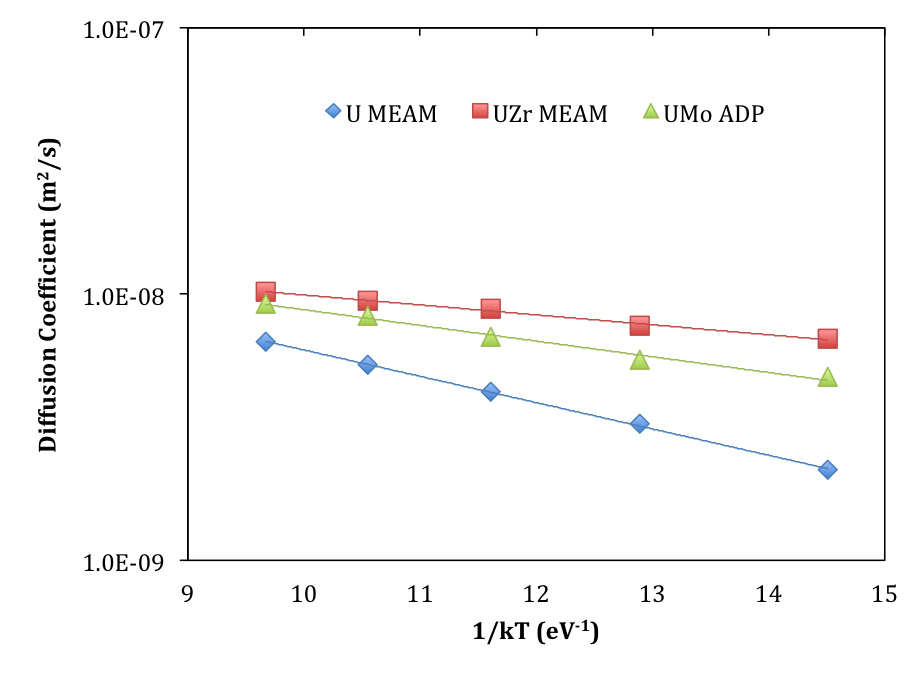
\includegraphics[width=0.8\textwidth]{diffa.png} % requires the graphicx package
 \caption{The interstitial diffusion coefficient in $\gamma$U for three different potentials from 800 K to 1200 K.}
 \label{fig:gamUdiff}
\end{figure}

\FloatBarrier

In a further attempt to understand this anomalous behavior, the calculation of elastic constants as a function of temperature from 800 K to 1200 K was performed. Typically, elastic constants soften as a function of temperature \cite{varshni1970}. If $\gamma$U exhibited anomalous elastic constant behavior versus temperature, this could perhaps contribute to the anomalous TDE as a function of temperature. Thus, elastic constants were calculated by performing displacements of the system and using the resultant changes in stress to compute the elastic stiffness tensor, as provided by the LAMMPS distribution. There exists a large amount of thermal fluctuation in these systems, leading to a large amount of noise in the elastic constant calculations. In spite of the thermal noise, clear trends can be obtained for the elastic constants as a function of temperature, given that robust enough sampling is performed. In order to achieve some statistical certainty for each simulation of elastic constants, 100 samples are taken, with a sampling interval of 10 timesteps. The systems are equilibrated for 100 ps, and the equilibrated run to obtain the stress tensor is 50 ps in length. This simulation produces the nine elastic constants. Given that the bcc system is cubic, C$_{11}$, C$_{22}$ and C$_{33}$ were averaged to obtain C$_{11}$. Similar averaging was performed to obtain C$_{12}$ and C$_{44}$. Six unique calculations were performed for each given temperature and interatomic potential in order to obtain averages of the elastic constants. This leads to the standard deviation across all systems of approximately plus or minus 5 GPa for a given elastic constant at a given temperature for a given potential. This is an acceptable amount of uncertainty to obtain quantitative values of the elastic constants and their respective trends as a function of temperature. The results of these simulations are displayed in Fig. \ref{fig:elastic}. The data points are overlaid with a linear fit to the data points to emphasize the trends in behavior versus temperature. There is some scatter in the data due to the fact that these are high temperature systems, but clear trends are observed. 

For all three potentials, there is a general softening of elastic constants as a function of temperature, as would be expected. Each potential shows a varying degree of softening with temperature, and the magnitude of the various elastic constants is not the same across all potentials. The most notable difference is the very low value of C$_{44}$ for the U MEAM potential. The bulk modulus is calculated as B=($C_{11}$+2$\times$C$_{12}$)/3. The bulk modulus as a function of temperature is shown in Fig. \ref{fig:bulk}. It is observed the UZr MEAM potential provides the most stiff elastic response, while U MEAM is the softest. This corresponds reasonably well to the relative magnitudes of the Frenkel pair formation energies for each of the potentials, with the UZr MEAM exhibiting the highest Frenkel pair formation energy and U MEAM the lowest. It is also observed the the UMo ADP exhibits the least amount of softening as a function of temperature. It is possible that the softening of elastic constants contributes to the reduction in the TDE as temperature increases, as a softer lattice would be more easily deformed.  

%Thus, anomalous behavior of elastic constants as a function of temperature can be ruled out as a contributing factor to the anomalous behavior of the TDE as a function of temperature. The full results of the elastic constants investigation are not included in this manuscript.

\begin{figure}[h]
 \centering
 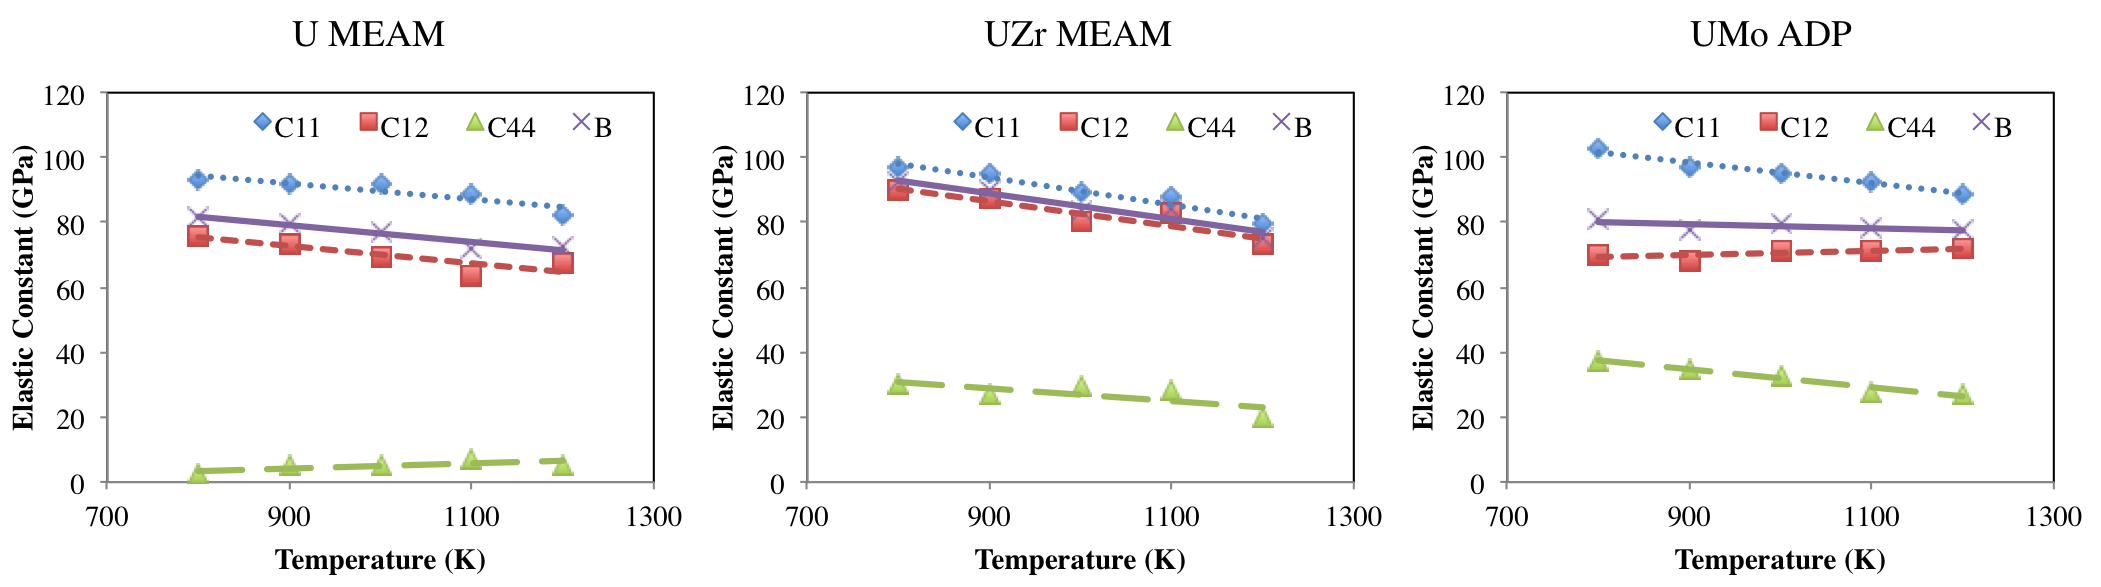
\includegraphics[width=\textwidth]{elastic_vs_T.png} % requires the graphicx package
 \caption{The elastic constants as a function of temperature in $\gamma$U for three different potentials from 800 K to 1200 K.}
 \label{fig:elastic}
\end{figure}

\begin{figure}[h]
 \centering
 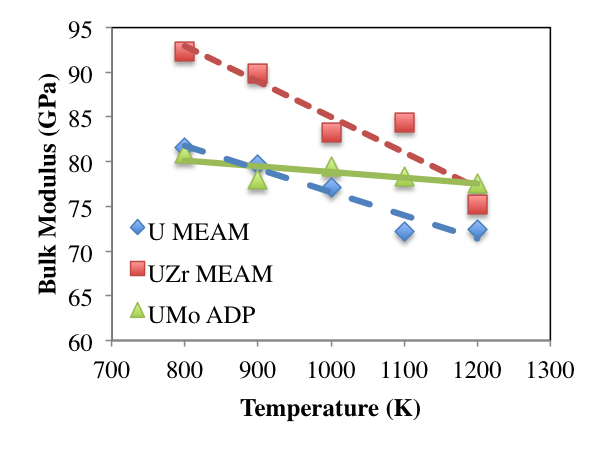
\includegraphics[width=0.8\textwidth]{bulk_vs_Ta.png} % requires the graphicx package
 \caption{The bulk modulus as a function of temperature in $\gamma$U for three different potentials from 800 K to 1200 K.}
 \label{fig:bulk}
\end{figure}

%At this point, although the specific reason is unclear, it is suspected that diffusion has an inverse relationship on TDE in $\gamma$U, which runs counter to previous investigations in other bcc materials. 

\subsubsection{Discussion of interatomic potential differences}

For further understanding of this system, the next step is to attempt to determine the cause of the discrepancies in the E$^{\textrm{pp}}_{\textrm{d,med}}$ between the potentials. In Fig \ref{fig:eform}, it is observed that UZr MEAM has the highest Frenkel pair formation energy across the temperature range investigated, while U MEAM exhibits the lowest Frenkel pair formation energy. Analyzing the interstitial diffusion coefficient across the entire temperature range in Fig \ref{fig:gamUdiff}, UZr MEAM exhibits the highest diffusion coefficient and the U MEAM exhibits the lowest diffusion coefficient. At 800 K, UZr has an interstitial diffusion coefficient three times larger than U MEAM. As temperature increases, the discrepancy between the diffusion coefficients narrows, as the UZr MEAM/U MEAM diffusion coefficient ratio at 1200 K is 1.5.  Finally, the elastic constants of all three potential soften as a function of temperature, with the magnitude of the bulk modulus loosely correlating to relative Frenkel pair formation energy.  

Within a given system, there are a variety of competing factors that influence the magnitude of the TDE. The interstitial formation energy should be positively correlated with the TDE, in that an increase in the formation energy leads to an increase in the TDE. The elastic constants should also be positively correlated with the TDE, in that a decrease in bulk modulus leads to a decrease in the TDE. Given the trends in the TDE across the potentials studied and the relative interstitial formation energies, a negative correlation between diffusion coefficient and threshold displacement energy is suggested, in that an increase in the diffusion coefficient leads to a decrease in the threshold displacement energy. This is in agreement with the comparison of the temperature dependence of the TDE given a single potential, and in opposition to the previous studies on Fe, as previously discussed. However, given these trends, the relative quantities of the TDE for each potential can be understood (relative in this context refers to the quantities of interest for one potential in relation to the other potentials utilized). Frenkel pair formation energies for the U MEAM and the UMo ADP are essentially the same, but since the UMo ADP potential has a higher interstitial diffusion coefficient, the threshold displacement energy is lower. The UZr MEAM potential has the highest Frenkel pair formation energies but also the highest interstitial diffusion coefficient, and yields the median threshold displacement energy among the potentials. All three potentials exhibit softening of elastic constants with increasing temperature, suggesting a decrease in the TDE. The resultant threshold displacement energy in $\gamma$U can be viewed as competition between formation energy, elastic properties and diffusion behaviors. 

One possible explanation for this anomalous behavior lies in the similarly anomalous diffusion behavior in $\gamma$U, in that self-diffusion is particularly high when compared to other bcc metals \cite{fedorov1978, smirnov1992}. This is largely due to role of interstitial atoms in self-diffusion, whereas typical self-diffusion in metals is a vacancy-mediated process. In systems such as bcc Fe (and other typical metals), the interstitial formation energy is much larger than the vacancy formation energy, and is typically in the range of 3-5 eV. In such systems, higher diffusion would lead to higher rates of annihilation when a Frenkel pair is created. In systems such as $\gamma$U, interstitials and vacancies exhibit similar formation energies, and these formation energies are much lower when compared to bcc Fe. Thus although there exists an energetic driving force for annihilation, the magnitude of such a driving force is much lower in $\gamma$U. Given this information, it can be understood that higher rates of diffusion can lead to transport of uranium atoms away from the thermal spike, increasing the likelihood of creating a defect. This would result in a lower TDE with increasing diffusion, analogous to increasing temperature. To the author's knowledge, no investigations into the TDE in $\beta$Zr or $\beta$Ti, which also exhibit anomalous diffusion similar to $\gamma$U, have been performed. Such a study could confirm or refute this postulation. 

It should be emphasized that this behavior is non-standard, but is consistent given each individual potential on its own, as well as a comparison of all three interatomic potentials together. This consistency in the anomalous behavior leads to the conclusion that it is in fact real. Regretfully, experiments cannot provide insight into this phenomena, as the TDE investigated via experimentation is restricted to the E$^{\textrm{l}}_{\textrm{d}}$ (which is not the quantity of interest investigated within this paper) and no such fundamental investigations into the TDE in metallic uranium have been performed.


\subsection{$\alpha$ U Median Threshold Displacement Energy}

In this section, E$^{\textrm{pp}}_{\textrm{d,med}}$ in $\alpha$ U is determined at 600 K and 800 K. This work utilized the UMo ADP interatomic potential \cite{smirnovaADP}. The probability of Frenkel pair production as a function of PKA energy is generated for each unique PKA direction. This leads to 64 unique probability curves for each interatomic potential. Similar to $\gamma$U in Fig \ref{fig:ed_dir}, there exists a strong dependence on the direction of the PKA. Whereas the system of $\gamma$U shown in Fig \ref{fig:ed_dir} shows a variance across PKA directions of approximately 70 eV, in the $\alpha$U system at 600 K there is an observed variance across directions of over 100 eV. Given that $\alpha$U is a more complex crystal system, high symmetry and low symmetry directions possess incredibly different characteristics and this is reflected in the stark variance across crystallographic directions for the PKA. The authors would again like to emphasize the importance of gathering a large set of PKA directions to accurately sample the entire phase space of the crystal structure of interest such that true average behavior can be approximated. 

The probability curves for all PKA directions are arithmetically averaged, creating a single angle-integrated probability curve for each of the three interatomic potentials. The angle-integrated probability curves at 600 K and 800 K are displayed in Fig. \ref{fig:alpha}. In Fig \ref{fig:alpha}, a line is overlaid on the data at a probability of 0.5 over the entire energy spectrum. The major observation from Fig. \ref{fig:alpha} is the minimal difference in the results from 600 K to 800 K. The value of E$^{\textrm{pp}}_{\textrm{d,med}}$ at 600 K is 65.5 eV and the value at 800 K is 64.5 eV, with no statistically significant differences observable. This suggests that in $\alpha$U, unlike $\gamma$U, any variance in defect energetics between 600 K and 800 K is compensated for via increased diffusion, yielding no discernible difference in the TDE.

\begin{figure}[h]
 \centering
 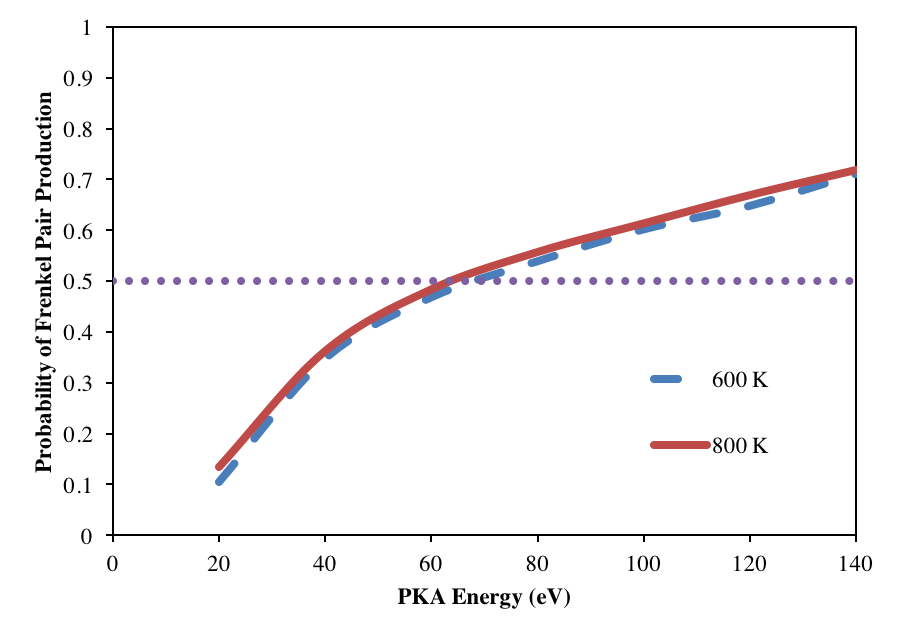
\includegraphics[width=0.8\textwidth]{alpha.png} % requires the graphicx package
 \caption{The angle-integrated Frenkel pair production probability curves at 600K and 800 K for $\alpha$U using the UMo ADP potential.}
 \label{fig:alpha}
\end{figure}

\FloatBarrier

To investigate defect behavior in $\alpha$ U, a set of simulations was conducted at 600 K and 800 K to ascertain the interstitial formation energy in $\alpha$U at each of these respective temperatures. Utilizing equation \ref{eqn:eint}, E$_{pure}$ and E$_{int}$ were determined by conducting ten unique simulations for a system with and without an interstitial. In each simulation, the system is equilibrated for 1 ns at a prescribed temperature, wherein the energy is averaged over the final 500 ps of the simulation. The resultant energy from each of the ten simulations was averaged to calculate E$_{pure}$ and E$_{int}$. It was found that the interstitial formation energy in $\alpha$U at 600 K is 2.57eV and at 800 K is 3.18 eV. The diffusion coefficients were also determined at 600 K and 800 K. Utilizing the same simulations that were conducted to determine interstitial formation energies, the mean square displacement was tracked as a function of time. The total simulation time of 1 ns was deemed to be sufficient as the diffusion coefficient had stabilized and \textit{r}$^{2}$ was linear with time. The calculated diffusion coefficients allowed for the determination of a migration barrier of 0.35 eV, which is slightly higher than the density functional theory value of 0.19 eV from Huang and Wirth \cite{wirth2011}. 

Finally, the results for $\alpha$U need to be compared to the results from $\gamma$U. Utilizing the same potential to compare two phases is the most direct way to approach this comparison, thus the results for only the UMo ADP interatomic potential \cite{smirnovaADP} will be discussed. At 800 K, $\alpha$U exhibits a TDE of 64.5 eV and $\gamma$U exhibits a TDE of 35.6 eV. Thus, it is much more probable for a PKA of a given energy to generate a defect in $\gamma$U than in $\alpha$U. This corresponds to the difference in interstitial formation energy between $\alpha$U and $\gamma$U for the UMo ADP potential, as the interstitial formation energy is 3.18 eV for $\alpha$U and 0.8 eV for $\gamma$U. In comparing the interstitial diffusion coefficients for $\alpha$ and $\gamma$U, interstitials diffuse approximately 3.5X faster in $\gamma$U. Given what we know about the relationship between diffusion and threshold displacement energy in $\gamma$U, this would further depress the relative value of TDE in $\gamma$U as compared to that from $\alpha$U. All of which is to say that the results from the defect analyses are in concordance with the threshold displacement energy simulation results, with the conclusion that a PKA of a given energy is more likely to produce a defect in $\gamma$U than in $\alpha$U. 

\FloatBarrier

\section{Conclusions}

In this study, molecular dynamics simulations were performed to calculate the threshold displacement energy in $\alpha$ and $\gamma$ U at 600 K, 800 K and 1000 K utilizing three unique interatomic potentials. The probability of Frenkel pair production was determined as a function of PKA direction and temperature. Probability curves are averaged to determine an effective value of the TDE, above which a Frenkel pair is more than 50 $\%$ likely to form. The value of TDE for $\gamma$U strongly depends on the interatomic potential utilized, as values range from 36 eV to 75 eV at 800 K. This is explained via the differences in interstitial formation energy and diffusion for each of the respective potentials. This also leads to the postulation that in $\gamma$U, TDE has a positive correlation with interstitial formation energy, but a negative correlation with diffusion coefficient. Finally, the TDE in $\alpha$U is found to be higher than in $\gamma$U. Thus, one would expect it to be more difficult to generate a defect in $\alpha$U than in $\gamma$U.


\section{Acknowledgement}
This work was supported by the U.S. High Performance Research Reactor (USHPRR) Fuel Qualification (FQ) Program 



\bibliography{MARMOTbib}


\end{document} 
